\documentclass[12pt,a4paper]{article}

\usepackage[utf8]{inputenc}
\usepackage[english]{babel}
\usepackage{amssymb, amsmath}
\usepackage{fullpage}
\usepackage{parskip}
\usepackage{url}

\usepackage{graphicx}
\usepackage{enumitem}

\usepackage[hidelinks]{hyperref}

\usepackage{xcolor,listings}


\lstset{
    commentstyle=\color{green},
    keywordstyle=\color{blue},
    numberstyle=\numberstyle,
    stringstyle=\color{red},
    basicstyle=\footnotesize\ttfamily,
    breakatwhitespace=false,
    breaklines=true,
    captionpos=b,
    keepspaces=true,
    showspaces=false,
    showstringspaces=false,
    showtabs=false,
    belowskip=-1\baselineskip,
}


\begin{document}
    SSP ``Homework''
    \hfill 
    R.~Andreev, \today
    
    %%%%%%%%%%%%%%%%%%%%%%%%%%%%%%
    \section{Funneling clicks through the widget}
    %%%%%%%%%%%%%%%%%%%%%%%%%%%%%%
    
    
    \subsection{Introduction}
    
    The aim of the task is to understand
    the ``funneling'' of clicks through 
    the size selection widget,
    in particular the difference
    between 
    \textbf{Partner A} and \textbf{Partner B}.
    %
    %
    %
    These events are encoded in 
    the \texttt{analytics.events} table
    in the \texttt{event\_name} field.
    %
    With the SQL query
    \begin{lstlisting}[language=SQL]
        select 
            event_name, 
            sum((partner_key = 'Partner A')::int) as "A", 
            sum((partner_key = 'Partner B')::int) as "B"
        from analytics.events
        group by event_name;
    \end{lstlisting}
    %
    we find the events shown in Table~\ref{t:ev_by_pk}.
    \begin{table}[p]
        \begin{center}
            \small
            \begin{tabular}{l|cc}
                \texttt{event\_name}     & Partner A & Partner B \\
                \hline
                viewed\_product          & 3492288 & 1842017 \\
                added\_variant\_to\_cart & 286695  & 130564  \\
                ordered\_variant         & 44962   & 23923  \\
                \hline
                opened\_editor           & 31073   & 6608    \\
                opened\_brand\_list      & 29478   & 8745    \\
                selected\_brand          & 16086   & 3928    \\
                selected\_category       & 3477    & 3488    \\
                selected\_size           & 12396   & 3302    \\
                completed\_profiling     & 12367   & 3291    \\
            \end{tabular}
        \end{center}
        %
        \caption{Summary of events by Partner.}
        \label{t:ev_by_pk}
    \end{table}
    
    %
    
    Playing with the widget, we infer the sequence of events
    we want to evestigate in detail as
    {
    
        \small
        \begin{enumerate}[itemsep=-1ex]
            \item \verb|opened_editor|
            \item \verb|opened_brand_list|
            \item \verb|selected_brand|
            \item \verb|selected_category|
            \item \verb|selected_size|
            \item \verb|completed_profiling|
        \end{enumerate}
    }

    %
    
    Let's break down the data 
    by \texttt{product\_domain}
    using the SQL query
    %
    \begin{lstlisting}[language=SQL]
        select product_domain, partner_key, count(event_name)
        from analytics.events
        group by product_domain, partner_key 
        order by product_domain, partner_key;
    \end{lstlisting}
    
    %
    
    The results are given in Table~\ref{t:pd_by_pk}.
    %
    %
    \begin{table}[p]
        \begin{center}
            \begin{tabular}{l|cc}
                \texttt{product\_domain} & {Partner A} & {Partner B} \\
                \hline
                Dresses          & 2982850   & 51771     \\
                Female Shoes     & 369043    & 409761    \\
                Female Tops      & 333421    & 134270    \\
                Female Bottoms   & 116141    & 45007     \\
                \hline
                Male Bottoms     & --        & 44183     \\
                Male Shoes       & --        & 105529    \\
                Male Tops        & --        & 140946    \\
                \hline
                Swimwear Bottoms & 18036     & --        \\
                Swimwear Tops    & 64358     & --        \\
                \hline
                NONE             & 44973     & 1094399  
            \end{tabular}
        \end{center}
        %
        \caption{Summary of products by Partner.}
        \label{t:pd_by_pk}
    \end{table}
    
    We see that {Partner A} and {Partner B}
    have significant portions of disjoin product domains. 
    %
    In addition, 
    the product domain ``Dresses'' 
    does have any 
    \verb|selected_category|
    events 
    (cf.~Table~\ref{t:ev_by_pk} and \S\ref{s:pd-dresses}). 
    %
    %
    Based on these observations,
    it makes more sense 
    to
    ``funnel'' the events
    \textbf{for each product domain separately}
    rather than in aggregate,
    which was requested in the assignment.
    

    \clearpage
    
    \subsection{Funnel by product domain}
    
    %
    
    To get the click rates by product domain
    we query as
    %
    \begin{lstlisting}[language=SQL]
        select event_name, count(event_name) as n
        from analytics.events
        where 
            (partner_key = '{partner_key}') and
            (product_domain LIKE '{product_domain}')
        group by event_name;
    \end{lstlisting}
    
    %
    
    For brevity,
    we only compare
    within the product domains 
    where both Partner A and Partner B are active:
    \begin{itemize}
    \item 
        ``Dresses'' (Figure~\ref{f:pd_dresses}),
    \item 
        ``Female Shoes'' (Figure~\ref{f:pd_shoes}),
    \item 
        ``Female Tops'' (Figure~\ref{f:pd_tops}),
    \item 
        ``Female Bottoms'' (Figure~\ref{f:pd_bottoms}).
    \end{itemize}

    %
    Three out of four
    show clearly higher rates
    for Partner B over Partner A.
    %
%     Taking 
%     \begin{itemize}
%     \item
%         all events or
%     \item 
%         only events with known product domain
%     \end{itemize}
%     results in similar rates.
    
    %
    
    \newpage
    
    \label{s:pd-dresses}
    
    \begin{figure}[p]
        \centering
        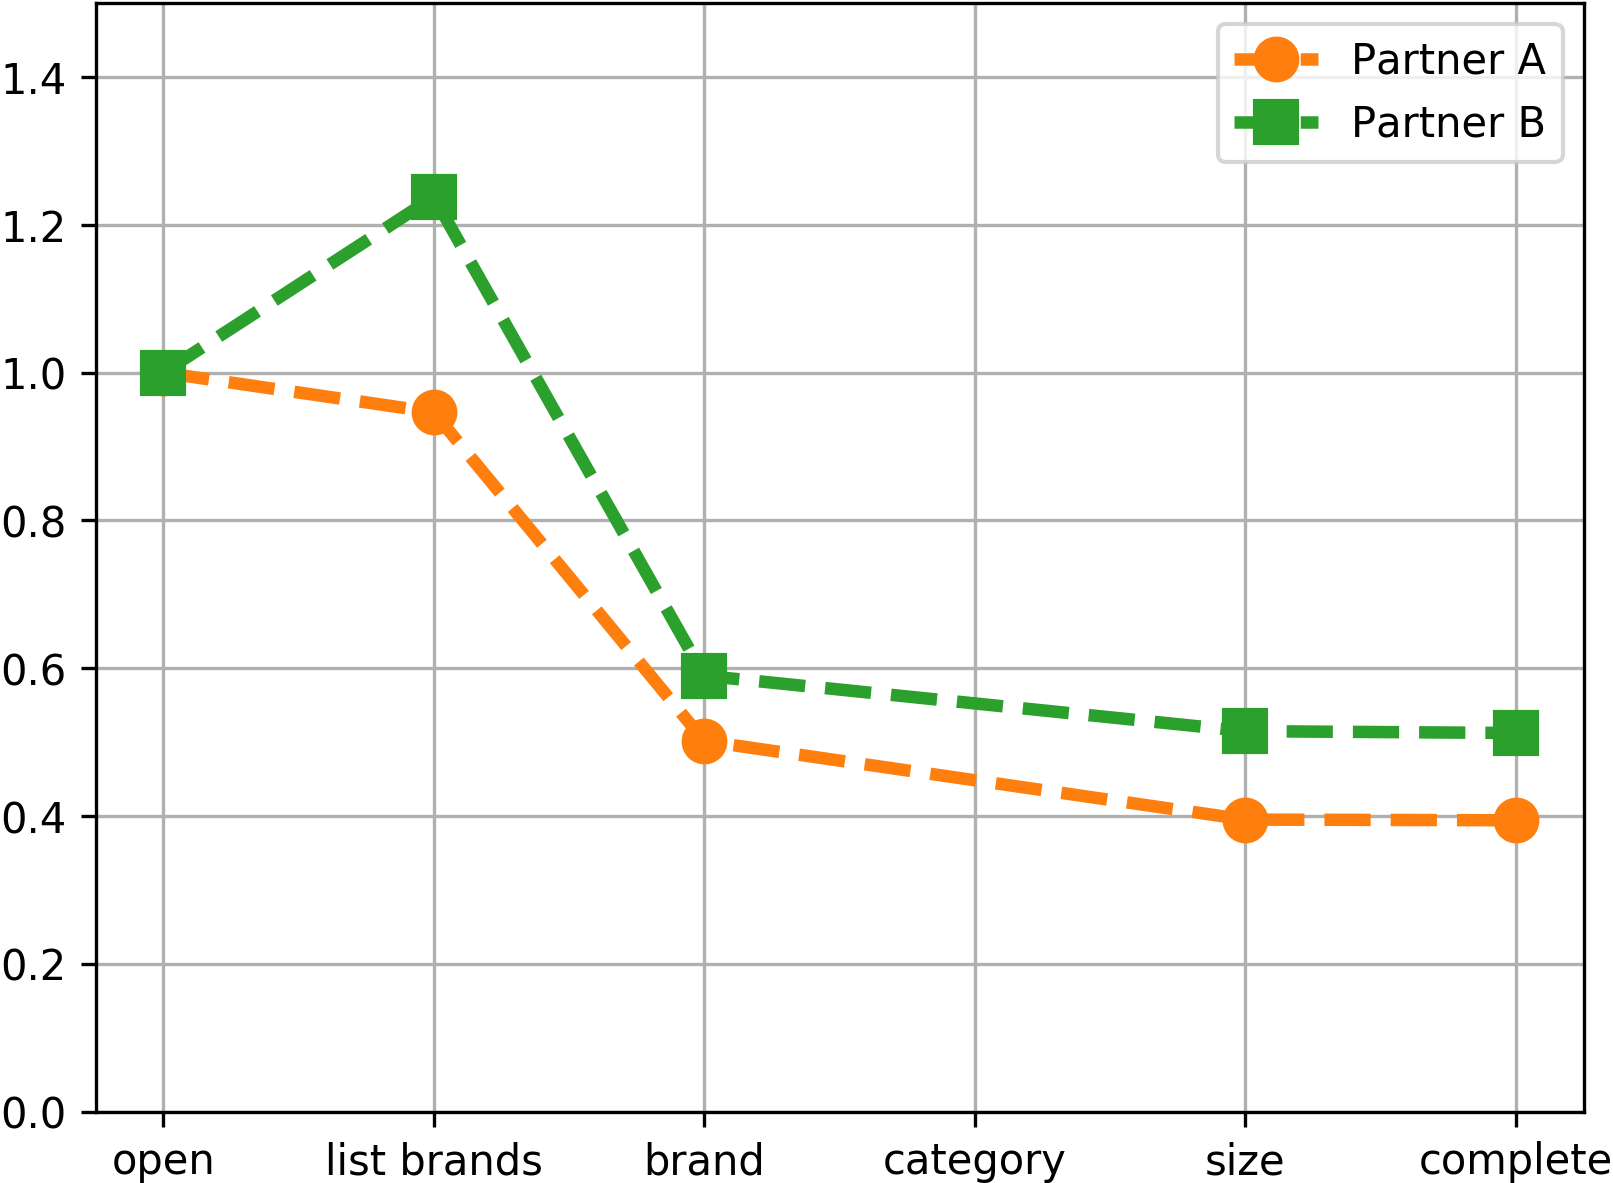
\includegraphics[width=0.8\textwidth]{../py/OUTPUT/funnel/img/product=Dresses.png}
        \caption{Funneling for product domain ``Dresses''.}
        \label{f:pd_dresses}
    \end{figure}

    
    \begin{figure}[p]
        \centering
        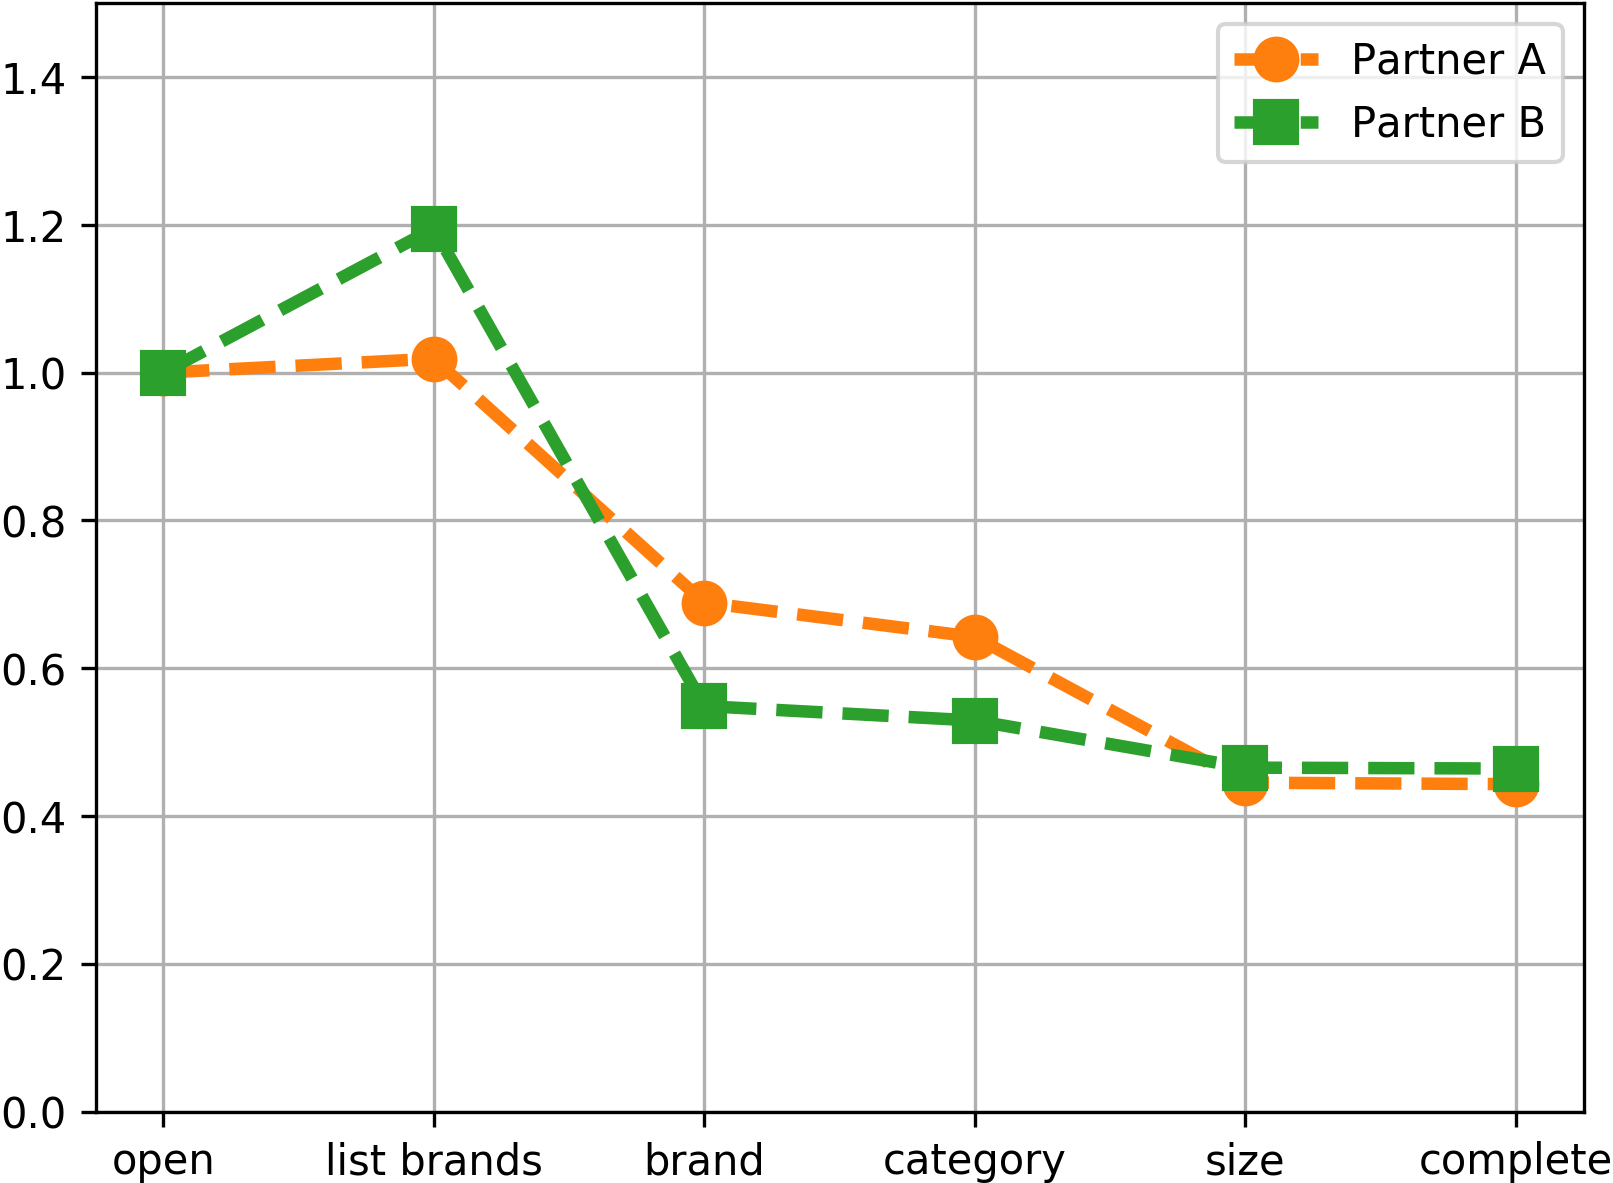
\includegraphics[width=0.8\textwidth]{../py/OUTPUT/funnel/img/product=Female_Shoes.png}
        \caption{Funneling for product domain ``Female Shoes''.}
        \label{f:pd_shoes}
    \end{figure}
    
    \begin{figure}[p]
        \centering
        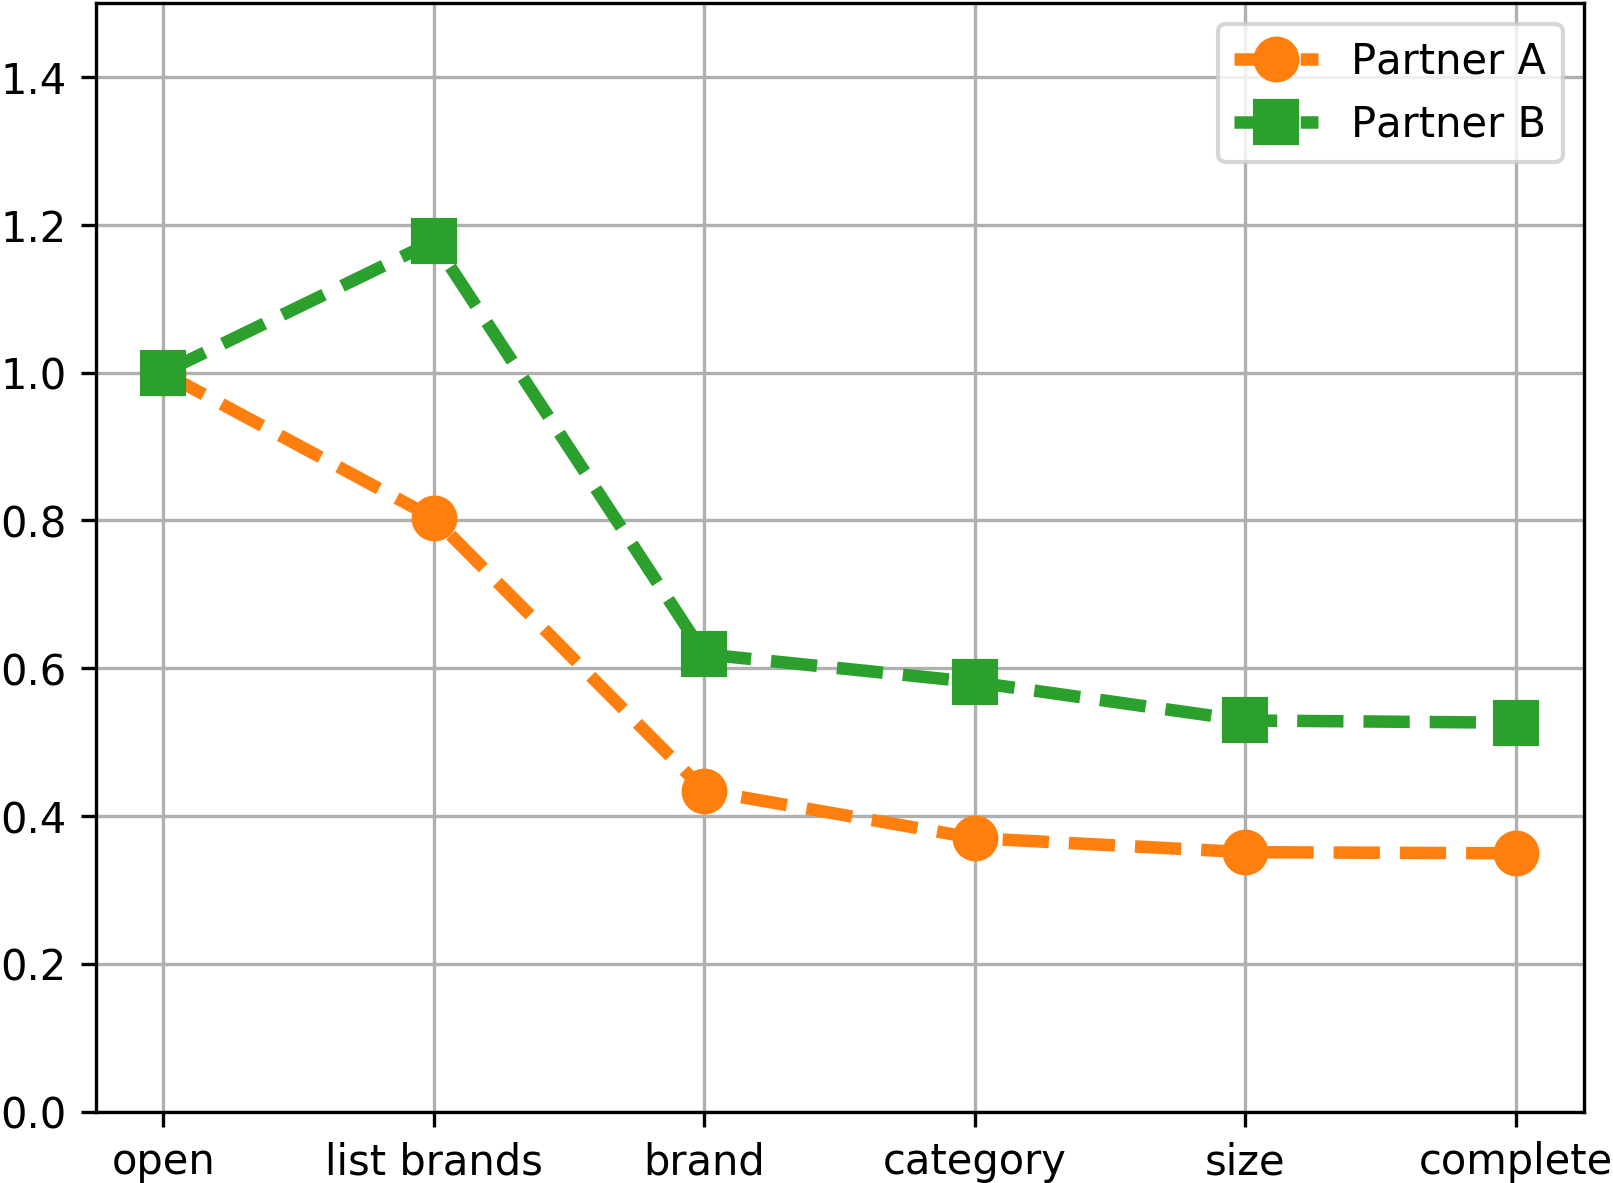
\includegraphics[width=0.8\textwidth]{../py/OUTPUT/funnel/img/product=Female_Tops.png}
        \caption{Funneling for product domain ``Female Tops''.}
        \label{f:pd_tops}
    \end{figure}
    
    \begin{figure}[p]
        \centering
        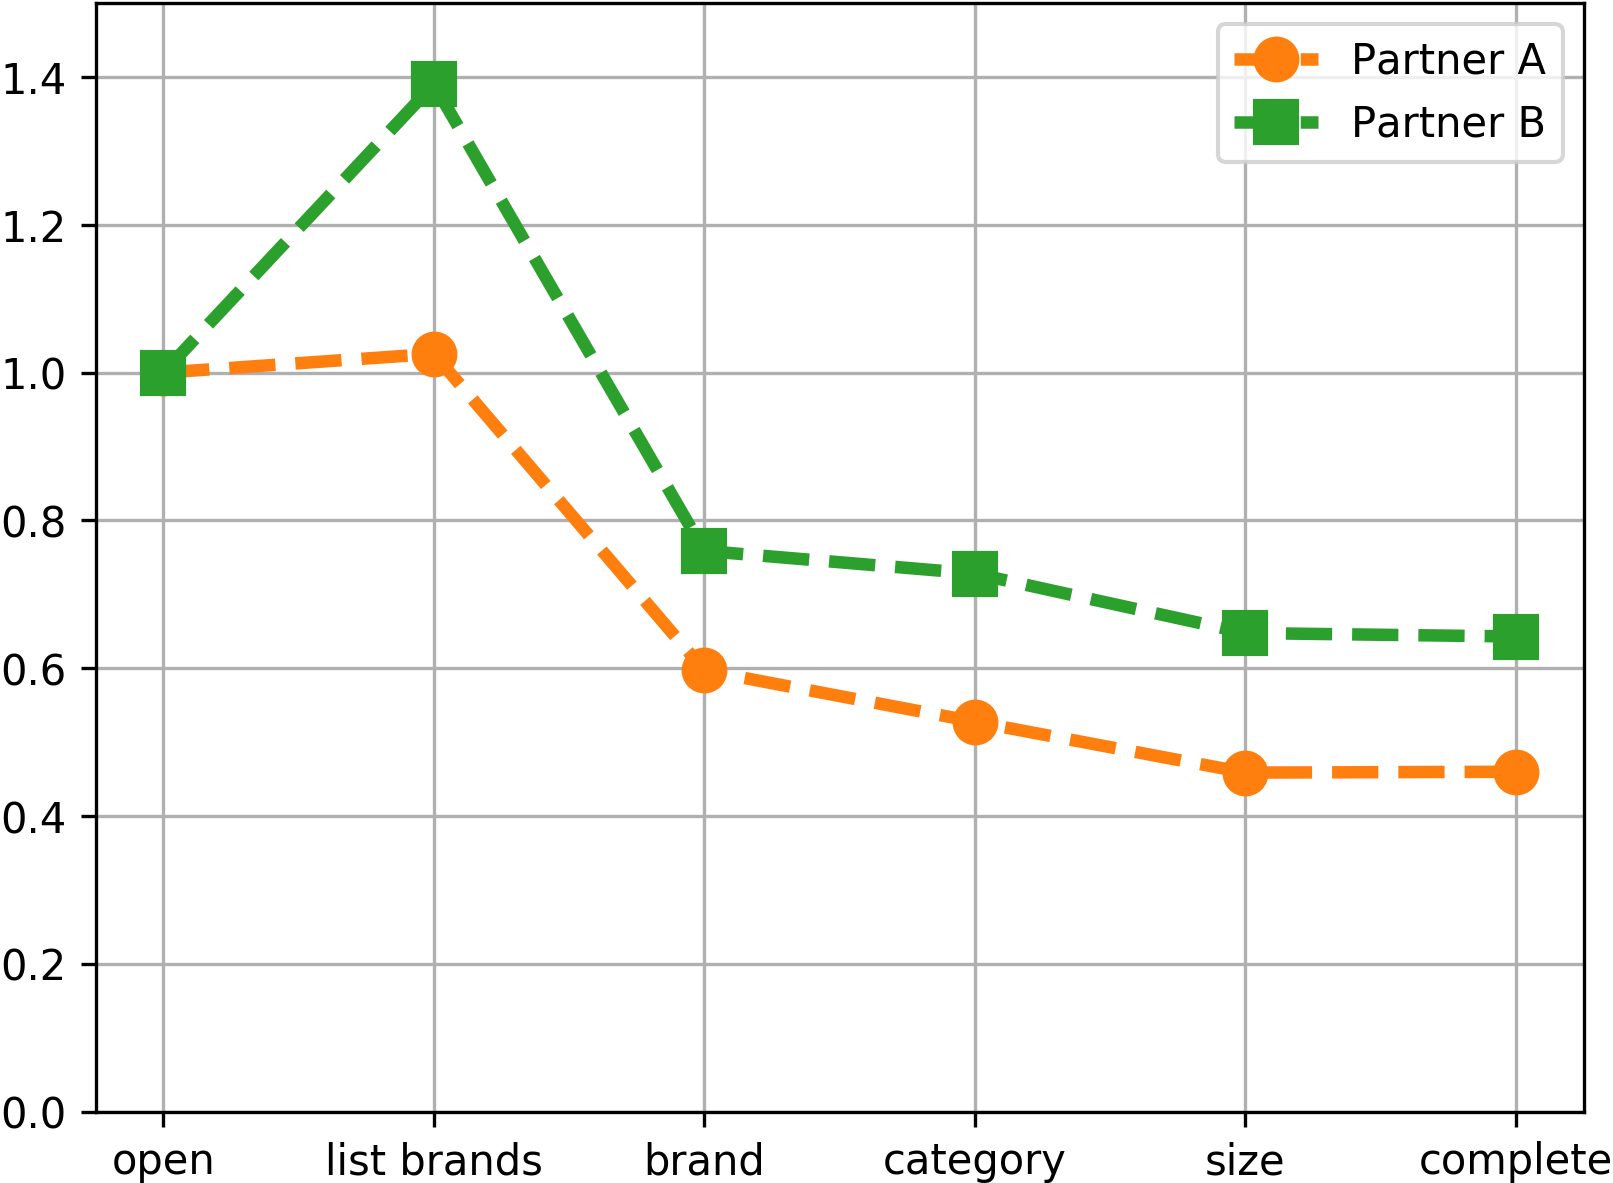
\includegraphics[width=0.8\textwidth]{../py/OUTPUT/funnel/img/product=Female_Bottoms.png}
        \caption{Funneling for product domain ``Female Bottoms''.}
        \label{f:pd_bottoms}
    \end{figure}
    
    
    \clearpage
    
    %%%%%%%%%%%%%%%%%%%%%%%%%%%%%%
    \section{Observations}
    %%%%%%%%%%%%%%%%%%%%%%%%%%%%%%
    
    \subsection{Higher funneling for B over A}
    
    The highlighted ones
    among product domains
    \begin{quote}
        \textbf{Dresses},
        Female Shoes,
        \textbf{Female Tops},
        \textbf{Female Bottoms}
    \end{quote}
    show clearly higher ``funneling'' rates
    for Partner B over Partner A.
    
    %
    
    Possible reasons are:
    %
    \begin{itemize}
    \item 
        the customer enters several purchased items
        via the ``add more'' button
        on website B
        because the meaning and appearance of 
        the button is clearer
        (assuming there is no \verb|opened_editor| event).
        %
        Compare, for example \textbf{revolve.com} and \textbf{farfetch.com}:
        \begin{center}
            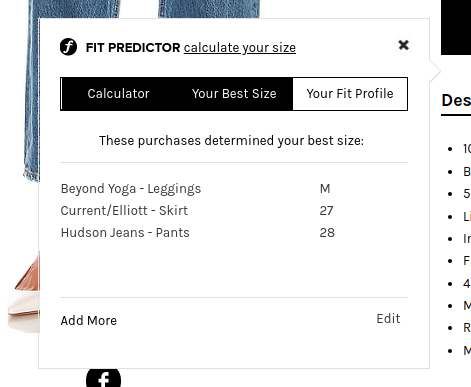
\includegraphics[width=0.42\textwidth]{../img/more_button/revolve}
            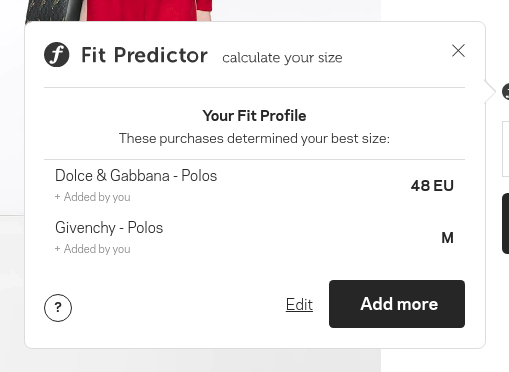
\includegraphics[width=0.48\textwidth]{../img/more_button/farfetch}
        \end{center}
    \item
        it is easier to 
        interact with the drop-down list of website B
        resulting in fewer misclicks.
    \item
        the widget implementation 
        is more robust on website B,
        i.e.~the widget is more likely to stall
        after the \verb|opened_editor| event
        on website A
        in some browsers.
    \end{itemize}

    %
    
    Non-reasons are:
    %
    \begin{itemize}
    \item
        the visibility of the widget,
        since the baseline is the \verb|opened_editor| event;
    \item
        male vs.~female customers, 
        since we are looking at dresses and such.
    \end{itemize}

    %
    
    \subsection{Sharp fall after \texttt{opened\_brand\_list} event}
    
    It appears that customers 
    click on the brand list inside the widget a lot,
    but then abandon the widget.
    %
    This is the case for both Partner A and Partner B.
    
    Possible reasons:
    
    \begin{itemize}
    \item
        They don't find the brands they own.
        %
        This creates a moment of confusion
        and the reflexive hope that 
        upon a second click
        the situation will be different.
        %
        Possibly,
        Partner B
        (with the high spike on \verb|opened_brand_list| event)
        is the fancier of the two
        (indeed, if it is \textbf{farfetch.com},
        that would be consistent with the earlier observation).
        
    \item
        They don't find \emph{another} brand they own
        after some successful entries.
    \item
        They don't remember the items or the sizes they own
        and have to look those up first, 
        i.e.~click on the brand list,
        close the list, look up item, open the list again.
    \end{itemize}

    
    \clearpage
    
    %%%%%%%%%%%%%%%%%%%%%%%%%%%%%%
    \section{Predicted size histogram}
    %%%%%%%%%%%%%%%%%%%%%%%%%%%%%%
    
    With the query
    %
    \begin{lstlisting}[language=SQL]
        select prediction_size, count(*) 
        from analytics.events 
        where 
            (partner_key = 'Partner A') and 
            (product_domain = 'Dresses') and 
            (event_name = 'completed_profiling') 
        group by prediction_size;
    \end{lstlisting}
    %
    we get 
    the predicted size 
    at
    the \verb|completed_profiling| event
    for dresses on Partner A's website.
    %
    %
    The results are in 
    Figure~\ref{f:pred_sz}.
    
    
    \begin{figure}[h]
        \qquad
        \begin{minipage}{0.55\textwidth}
            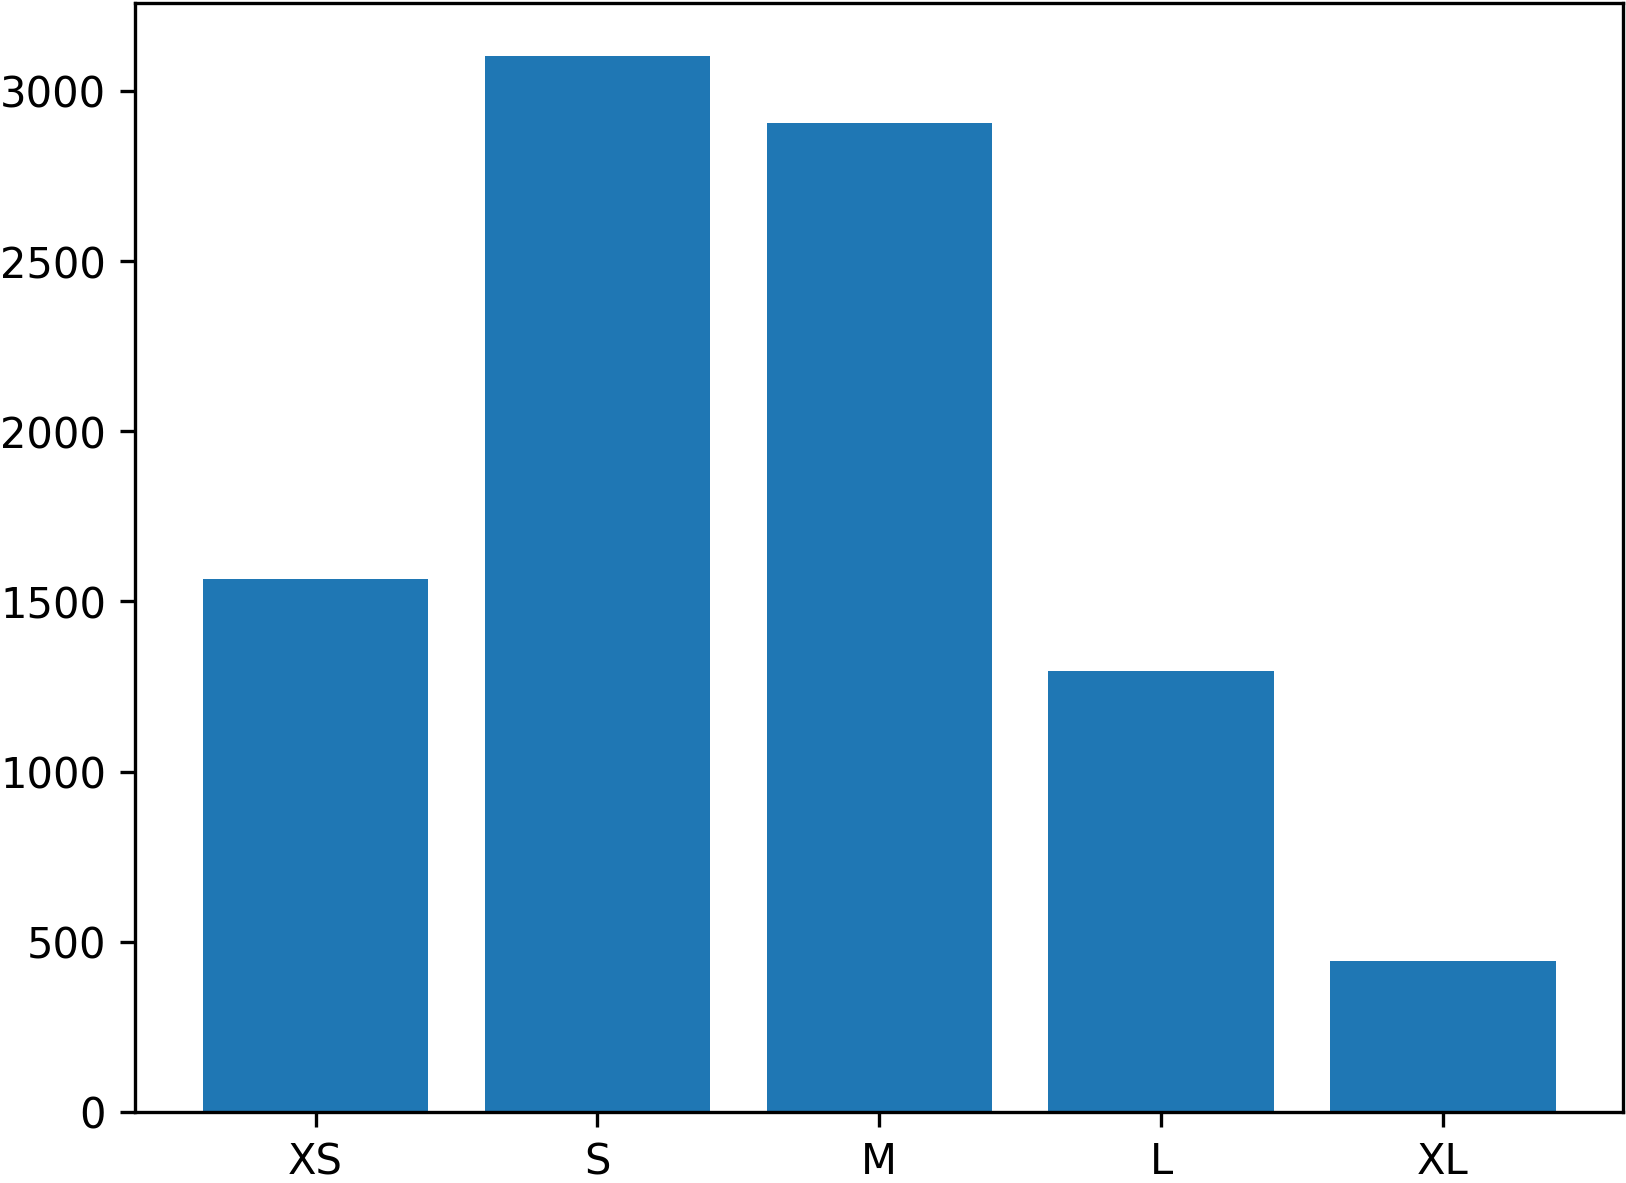
\includegraphics[width=\textwidth]{../py/OUTPUT/histo/img/histo.png}
        \end{minipage}
        \hfill
        \begin{minipage}{0.3\textwidth}
            \small
            \begin{tabular}{c|c}
                \verb|prediction_size| & \# \\
                \hline
                12  & 1    \\
                2   & 3    \\
                4   & 6    \\
                6   & 2    \\
                8   & 3    \\
                L   & 1296 \\
                M   & 2905 \\
                S   & 3103 \\
                XL  & 442  \\
                XS  & 1566 \\
                XXS & 6    \\
                NULL & 232 
            \end{tabular}
        \end{minipage}
        \qquad
        
        \caption{Predicted size distribution for dresses of Partner A.}
        \label{f:pred_sz}
    \end{figure}
    
    
    \clearpage
    
    %%%%%%%%%%%%%%%%%%%%%%%%%%%%%%
    \section{A/B testing}
    %%%%%%%%%%%%%%%%%%%%%%%%%%%%%%
    
    Does the fit predictor make more people purchase the products?
    %
    Presumably,
    the purchase of a product is indicated 
    by
    the \verb|ordered_variant| event.
    %
    We can compare the number of those events 
    to the number of \verb|viewed_product| events
    (or, alternatively, to \verb|added_variant_to_cart| events,
    but the results are similar).
    %
    So we define the conversion rate 
    as
    \begin{align}
        \textrm{conversion rate}
        =
        \frac{ 
            \#\mathtt{ordered\_variant}
        }{
            \#\mathtt{viewed\_product}
        }
        .
    \end{align}
    
    With the query
    \begin{lstlisting}[language=SQL]
        select 
            event_name, 
            sum((ab_slot1_variant = 'Control')::int) as "Control", 
            sum((ab_slot1_variant = 'Test')::int) as "Test" 
        from analytics.events 
        where 
            (partner_key = 'Partner A') 
            and
            (
                (event_name = 'viewed_product') or 
                (event_name = 'ordered_variant')
            )
        group by event_name;
    \end{lstlisting}
    %
    we get the table
    %
    \begin{center}
        \begin{tabular}{l|cc}
            event\_name      & Control & Test    \\
            \hline
            viewed\_product  & 1749420 & 1742868 \\
            ordered\_variant & 22156   & 22806  \\
            \hline
            conversion rate & 0.012665 & 0.013085
        \end{tabular}
    \end{center}
    %
    of the pertinent events 
    for the Control and Test groups,
    where we have added the conversion rate by hand.
    %
    The conversion rate has increased in the Test group.
    %
    Next, we test the statistical significance of the improvement.
    
    
    \subsection{Binomial test}
    
    Our null-hypothesis is:
    a customer purchases a viewed product
    with the probability $p$.
    %
    This probability
    is determined from the Control group.
    %
    % p = (22156 / 1749420)
    %
    Let $p'$ denote the corresponding probability
    for the Test group.
    %
    % p' = (22806 / 1742868)
    %
    We wish to check if $p' > p$ is significant.
    %
    Since the number of observations 
    $n'$
    % n' = (1742868)
    in the Test group is rather large
    (although $p'$ is somewhat small),
    we resort to the normal approximation
    and
    compute the z-score:
    %
    \begin{align}
        z
        =
        \frac{
            p' - p
        }{
            \sqrt{ p (1 - p) / n' }
        }
        \approx
        4.965
        .
    \end{align}
    %
    This gives an $\alpha$-value of 
    $\alpha \approx 3.43 \times 10^{-7}$.
    %
    %
    The observed improvement 
    in the conversion rate
    is 
    therefore
    highly statistically significant.
    
    This reasoning is contaminated
    by multiple visits 
    by the same user in a session
    to the website,
    mainly because the number is unequal among users.
    %
    It would be cleaner to identify those visits as one.
    
    
    \subsection{Fisher test}
    
    For the Fisher $2 \times 2$ test we rephrase the table as
    %
    \begin{center}
        \begin{tabular}{l|cc}
            ordered & Control & Test    \\
            \hline
            no & 1727264 & 1720062 \\
            yes & 22156   & 22806  
        \end{tabular}
    \end{center}
    %
    by considering the complement 
    of \verb|ordered_variant| event as
    the no-order case.
    %
    %
    %
    Aforegoing remarks on contamination by 
    multiple visits
    apply.
    %
    Nevertheless,
    the Fisher exact test statistic value is 0.05\%,
    again highly statistically significant.
    
    
    
    %%%%%%%%%%%%%%%%%%%%%%%%%%%%%%
    \section*{Appendix}
    %%%%%%%%%%%%%%%%%%%%%%%%%%%%%%
    
    The Python codes are deposited under
    \begin{quote}
        \url{https://github.com/numpde/misc/tree/master/ssp}
    \end{quote}

\end{document}

